\documentclass[11pt,a4paper]{ctexart}
\usepackage[a4paper,margin=1.8cm,headheight=14pt]{geometry}
\usepackage{amsmath,amssymb,mathtools}
\usepackage{booktabs,tabularx,longtable,array,multirow}
\usepackage{enumitem}
\usepackage{tikz}
\usetikzlibrary{arrows.meta,positioning,shapes.geometric,fit,calc}
\usepackage[most]{tcolorbox}
\usepackage{xcolor}
\usepackage{fancyhdr}
\usepackage{hyperref}
\usepackage{microtype}
\setlength{\parindent}{2em}
\setlength{\parskip}{0.35em}
\setlist[itemize]{itemsep=0.2em,topsep=0.3em}
\setlist[enumerate]{itemsep=0.2em,topsep=0.3em}
\hypersetup{colorlinks=true,linkcolor=blue!45!black,urlcolor=blue!50!black}

\definecolor{mainblue}{RGB}{45,86,140}
\definecolor{deepblue}{RGB}{30,62,102}
\definecolor{softblue}{RGB}{238,245,252}
\definecolor{softgreen}{RGB}{238,249,243}
\definecolor{softorange}{RGB}{253,246,233}
\definecolor{softred}{RGB}{253,239,239}
\definecolor{softgray}{RGB}{246,247,249}
\definecolor{deepgreen}{RGB}{35,105,75}
\definecolor{deeporange}{RGB}{165,98,22}
\definecolor{deepred}{RGB}{150,55,55}

\pagestyle{fancy}
\fancyhf{}
\lhead{408 操作系统方法论}
\rhead{OS-00 基础与程序运行环境}
\cfoot{\thepage}
\renewcommand{\headrulewidth}{0.4pt}

\newtcolorbox{corebox}[1][]{colback=softblue,colframe=mainblue,title=#1,fonttitle=\bfseries,boxrule=0.8pt,arc=2mm}
\newtcolorbox{exam}[1][]{colback=softorange,colframe=deeporange,title=#1,fonttitle=\bfseries,boxrule=0.8pt,arc=2mm}
\newtcolorbox{warn}[1][]{colback=softred,colframe=deepred,title=#1,fonttitle=\bfseries,boxrule=0.8pt,arc=2mm}
\newtcolorbox{eng}[1][]{colback=softgreen,colframe=deepgreen,title=#1,fonttitle=\bfseries,boxrule=0.8pt,arc=2mm}
\newtcolorbox{method}[1][]{colback=softgray,colframe=black!45,title=#1,fonttitle=\bfseries,boxrule=0.6pt,arc=2mm}

\newcommand{\kw}[1]{\textbf{#1}}
\newcommand{\code}[1]{\texttt{#1}}

\title{\vspace{-1.2cm}\textbf{操作系统基础与程序运行环境}\\[0.4em]
\large 从裸硬件到受保护、可共享、可管理的执行环境}
\author{408 操作系统专题手册 OS-00}
\date{}

\begin{document}
\maketitle

\begin{corebox}[母问题：操作系统为什么存在？]
\begin{center}
\Large\bfseries 一段普通程序为什么可以像“独占一台机器”一样运行，\\
而真实硬件明明有限、共享、异步，并且可能发生故障？
\end{center}

本册不从“操作系统有哪些功能”开始背诵，而从\kw{裸硬件不能直接满足程序需求}开始推导：
\[
\boxed{
\text{Finite Physical Resources}
\xrightarrow[\text{Protection + Policy}]{\text{Abstraction + Virtualization}}
\text{Program-visible Managed Environment}
}
\]

全书继续沿用 OS 统一推演引擎：
\[
\boxed{
\text{State}\to\text{Transition}\to\text{Failure}\to\text{Property}\to\text{Mechanism}\to\text{Tradeoff}
}
\]
但 OS-00 的任务不是深入某个局部机制，而是建立后续所有 Topic 共用的\kw{坐标系、运行入口和边界}。
\end{corebox}

\begin{method}[术语预备：本册先固定这些词的含义]
\begin{itemize}[leftmargin=1.5em]
  \item \kw{操作系统 (OS)}：运行在硬件之上、为程序分配资源并提供受保护接口的软件系统；它不是某个单独的应用程序。
  \item \kw{抽象 (Abstraction)}：隐藏硬件实现细节，只向程序暴露稳定的对象和操作，例如把磁盘块组织成可按名字打开的文件。
  \item \kw{虚拟化 (Virtualization)}：用软件和硬件把有限物理资源表示成多个彼此隔离的逻辑资源，例如每个进程看到自己的虚拟地址空间。
  \item \kw{保护/隔离 (Protection/Isolation)}：规定一个执行主体能访问哪些对象，并阻止它越过权限边界修改其他主体的状态。
  \item \kw{资源管理 (Resource Management)}：在资源有限或多人竞争时，负责分配、回收、复用和调度 CPU、内存、设备及存储。
  \item \kw{用户态/内核态 (User/Kernel Mode)}：CPU 的两种权限状态。用户态不能执行特权操作；内核态可以管理页表、设备和调度状态。
  \item \kw{系统调用 (System Call)}：用户程序请求 OS 服务的受控入口，例如 \code{read}、\code{open} 和 \code{fork}；它不是普通函数调用。
  \item \kw{中断 (Interrupt)}：由当前指令流之外的硬件事件异步通知 CPU；\kw{异常 (Exception)}：由当前指令或执行结果同步触发的控制转移。
  \item \kw{引导 (Boot)}：机器上电后由固件和引导程序逐步装入内核、建立最小运行环境并交出控制权的过程。
\end{itemize}
这些词后文若出现缩写，均沿用这里的含义；具体机制由 OS-01/02 至 OS-06/07 分册展开。
\end{method}

\begin{method}[Owner / Stop Boundary]
本册完整拥有：OS 基本概念、发展逻辑、408 四特征、程序链接与装入的入口语义、运行时映像的基础区分、OS 结构、系统引导、机器级虚拟化，以及这些概念与后续 Topic 的导航关系。

以下内容只给\kw{最小接口}，不重新拥有内部机制：
\begin{itemize}
  \item user/kernel mode、system call、exception、interrupt 的控制权细节 $\rightarrow$ OS-01/02；
  \item 同步互斥、PV、管程、死锁 $\rightarrow$ OS-03；
  \item 地址翻译、页表、缺页、页置换、COW/mmap $\rightarrow$ OS-04；
  \item driver、DMA、I/O request、buffering、device scheduling $\rightarrow$ OS-05；
  \item pathname、fd/OFD、inode、文件分配与一致性 $\rightarrow$ OS-06/07；
  \item 特权级、MMU、IRQ controller 的硬件实现 $\rightarrow$ CPU $\times$ OS Bridge。
\end{itemize}
\end{method}

\tableofcontents
\newpage

\section{第一章：从裸机到可用机器——程序需要哪些服务}

\subsection{从一条指令开始：裸机模型看起来很简单}

若只从 CPU 的视角观察，一个正在运行的程序似乎只是不断重复：
\[
\boxed{\text{Fetch}\rightarrow\text{Decode}\rightarrow\text{Execute}}
\]
程序读写内存、执行算术、分支和函数调用，直到结束。

问题在于：\kw{这只描述了单个程序在理想机器上的局部执行，不描述真实系统怎样让很多程序安全、方便、有效地共享同一套硬件。}

把真实机器放回来，立刻出现四组矛盾：

\begin{enumerate}
  \item \kw{资源有限}：CPU 核心、内存、设备和持久存储都有限；
  \item \kw{多个程序竞争}：多个程序同时想用 CPU、RAM 和设备；
  \item \kw{直接访问危险}：任何程序若可任意修改页表、设备控制寄存器或别人的内存，隔离立即失效；
  \item \kw{硬件接口复杂且异步}：设备速度不同，完成事件可能在程序执行的任意时刻到来。
\end{enumerate}

因此程序不直接操作某块裸硬件，而是通过操作系统提供的接口使用 CPU、内存、文件和设备；内核同时检查权限并隔离不同程序。

\begin{corebox}[第一条生成链：操作系统的双视角 (Twin Viewpoint)]
\[
\boxed{
\text{OS} = \text{Resource Manager} + \text{Extended Machine / Interface}
}
\]
分析操作系统的任何功能时，固定从双重视角看：
\begin{enumerate}
  \item \kw{自下而上：资源管理者 (Resource Manager)}：面对物理硬件（CPU、内存、设备、磁盘），负责分配、复用、隔离与并发管控；
  \item \kw{自上而下：扩展机与抽象层 (Extended Machine / Interface)}：面向应用程序，隐藏底层接口细节，把粗糙的物理硬件重新解释为优雅的逻辑抽象（进程、虚拟内存、文件、系统调用）。
\end{enumerate}
\end{corebox}

\subsection{Abstraction：先把“怎么做”隐藏成“我能做什么”}

硬盘提供块、扇区和控制命令，应用却按\code{/home/a.txt}访问文件。物理内存是一串字节位置，程序却使用自己的虚拟地址。CPU 数量有限，调度器则让多个执行流轮流获得处理器时间。

因此第一层不是虚拟化，而是\kw{抽象（Abstraction）}：
\[
\boxed{\text{Complex Physical Interface}\rightarrow\text{Stable Logical Interface}}
\]

典型例子：
\begin{center}
\small
\renewcommand{\arraystretch}{1.25}
\begin{tabularx}{0.92\linewidth}{>{\bfseries}p{0.22\linewidth} p{0.28\linewidth} X}
\toprule
物理资源 & 程序希望看到的抽象 & 后续 Owner\\
\midrule
CPU & process / thread、可运行执行流 & OS-01/02\\
内存 & address space、可保护的虚拟地址 & OS-04\\
存储设备 & file / directory / namespace & OS-06/07\\
I/O 设备 & 统一或受控的 I/O interface & OS-05\\
\bottomrule
\end{tabularx}
\end{center}

\begin{warn}[Abstraction $\neq$ Virtualization]
抽象回答：\kw{“程序应该通过什么对象和接口使用资源？”}

虚拟化回答：\kw{“怎样让有限物理资源表现得像更丰富、可独立使用的逻辑资源？”}

两者经常一起出现，但不能当作同义词。
\end{warn}

\subsection{Virtualization：把有限资源变成多个可管理的逻辑实例}

OSTEP 将 virtualization 作为 OS 的核心组织原则之一：OS 接收 CPU、memory、disk 等物理资源，把它们转化成更通用、更方便使用的虚拟形式，同时通过 mechanism 与 policy 决定怎样共享这些资源。

最直观的例子是 CPU：只有少量 CPU 核心，却能让大量程序都表现为“正在运行”。这不是凭空创造算力，而是：
\[
\boxed{
\text{Physical CPU Time}
\xrightarrow{\text{Multiplexing + State Preservation}}
\text{Many Logical Execution Streams}
}
\]

内存同理：
\[
\boxed{
\text{Physical Memory}
\xrightarrow{\text{Mapping + Protection}}
\text{Per-process Address Spaces}
}
\]

\begin{exam}[题目信号]
看到“多个进程都认为自己从同一虚拟地址开始”“单核却有多个程序同时运行”“逻辑资源数量大于物理资源数量”时，第一动作不是背算法，而是问：
\[
\boxed{\text{物理资源是什么？虚拟对象是什么？谁负责映射和复用？}}
\]
\end{exam}

\subsection{Protection / Isolation：虚拟化必须带权限边界}

如果只是“共享”，没有隔离，一个程序就能破坏另一个程序或内核。因此：
\[
\boxed{\text{Sharing without Protection}\Rightarrow\text{Unsafe System}}
\]

OS 必须控制：
\begin{itemize}
  \item 哪些指令普通程序不能直接执行；
  \item 哪些地址可以访问；
  \item 哪些资源对象具有访问权限；
  \item 哪些状态只能由内核修改。
\end{itemize}

Protection 是后续 user/kernel mode、memory protection、file permission、capability 等机制共享的上位问题。本册只建立这个目标，不在这里展开硬件特权级和具体权限实现。

\subsection{Resource Management：虚拟化之后还必须决定“谁先用、用多少”}

当多个程序竞争同一资源时，仅有 mechanism 不够，还需要 policy：
\[
\boxed{\text{Mechanism: 能不能做？}\qquad\text{Policy: 选择谁做？}}
\]
例如：
\begin{itemize}
  \item CPU 可以被切换，这是 mechanism；下一位运行谁，是 scheduling policy；
  \item 页面可以被换出，这是 mechanism；淘汰哪一页，是 replacement policy；
  \item 磁盘请求可以排队，这是 mechanism；下一请求选谁，是 device scheduling policy。
\end{itemize}

这解释了 OS 为什么也被称为\kw{resource manager}。

\subsection{OS 的功能与服务：不要再背“处理机/存储器/文件/设备管理”四张孤立卡片}

传统教材常把 OS 功能列成处理机管理、存储器管理、文件管理、设备管理，再补用户接口。更好的挂法是按\kw{资源域 + 对外服务}理解：

\begin{center}
\small
\renewcommand{\arraystretch}{1.25}
\begin{tabularx}{\linewidth}{>{\bfseries}p{0.20\linewidth} p{0.28\linewidth} X}
\toprule
资源/对象域 & OS 必须解决的母问题 & 后续 Owner\\
\midrule
CPU / execution & 谁能运行、何时运行、怎样保存/恢复执行上下文 & OS-01/02\\
shared state & 多个执行流交错时怎样保持正确性与进展 & OS-03\\
memory & 地址空间、分配、保护、驻留和回收怎样管理 & OS-04\\
I/O device & 请求怎样提交、等待、完成并与设备速度差异解耦 & OS-05\\
persistent storage & 名字、对象、内容、空间和崩溃后一致性怎样维持 & OS-06/07\\
\bottomrule
\end{tabularx}
\end{center}

从应用视角，OS 还必须提供\kw{可调用接口}：程序执行、I/O、文件/目录操作、通信、错误处理、资源分配、保护等最终通过 API / system-call boundary 暴露。这里要保持：
\[
\boxed{\text{Library API}\neq\text{System Call}\neq\text{Kernel Internal Function}}
\]
一个库函数可能完全在用户态完成，也可能封装一个或多个 system calls；system call 是受控进入内核服务的接口语义。

\begin{exam}[功能题第一动作]
题目问“操作系统功能/服务”时，先问它在管理哪个\kw{资源域}、向谁提供什么\kw{可观察接口}，再把它送到后续 Owner。不要把“管理功能”和“用户接口”混成同一层。
\end{exam}

\section{第二章：OSTEP 三条主线与 408 四特征——两套坐标，不要硬凑}

\subsection{OSTEP 的 Three Easy Pieces 是三类“系统问题”}

OSTEP 用三条主线组织操作系统：
\[
\boxed{\text{Virtualization}+\text{Concurrency}+\text{Persistence}}
\]

它们分别追问：
\begin{enumerate}
  \item \kw{Virtualization}：怎样把 CPU、memory 等物理资源变成可共享的逻辑资源？
  \item \kw{Concurrency}：多个活动同时推进时，交错和共享状态怎样保持正确？
  \item \kw{Persistence}：数据怎样跨越进程生命周期和断电继续存在？
\end{enumerate}

它们是\kw{课程组织轴 / 问题轴}，不是 408 四特征的英文翻译。

\subsection{408 四特征描述的是 OS/多道环境呈现出来的性质}

\begin{center}
\small
\renewcommand{\arraystretch}{1.25}
\begin{tabularx}{\linewidth}{>{\bfseries}p{0.14\linewidth} p{0.24\linewidth} X}
\toprule
特征 & 判断依据 & 容易混淆的概念\\
\midrule
并发 & 多个事件在一段时间内交替推进 & 并发 $\neq$ 并行；单核也可并发\\
共享 & 多个执行实体共同使用有限资源 & 互斥共享与同时共享不同\\
虚拟 & 物理实体被变换成逻辑上的多个/更易用实体 & 虚拟 $\neq$ “不存在”\\
异步 & 进程推进速度和完成时刻具有不可预知性 & 异步来自调度、竞争、设备完成等不确定交错\\
\bottomrule
\end{tabularx}
\end{center}

\subsection{四特征的因果关系比并列背诵更重要}

不要把四个词当四张卡片。更好的生成关系是：
\[
\boxed{
\text{有限资源被共享}
\Rightarrow
\text{多个活动并发推进}
\Rightarrow
\text{执行次序和进度呈异步性}
}
\]
同时，为了让共享更方便、安全，OS 使用虚拟化：
\[
\boxed{
\text{Physical Sharing}
\xrightarrow{\text{Virtualization + Protection}}
\text{Logical Isolation / Managed Sharing}
}
\]

\begin{exam}[边界辨析]
\begin{itemize}
  \item \kw{并发 $\neq$ 并行}：并发强调时间段内多个活动都在推进；并行强调同一时刻同时执行。
  \item \kw{共享是并发的资源条件之一}：若完全没有资源关系，很多并发冲突就不会出现。
  \item \kw{异步不是“使用异步 I/O”}：它是更一般的推进次序不确定性。
  \item \kw{虚拟不是模拟器专属术语}：CPU 时间复用、地址空间、文件抽象都体现广义虚拟化思想。
\end{itemize}
\end{exam}

\subsection{虚拟化按什么维度复用？异步又逼出什么正确性底线？}

在 408 的经典分类中，“把一个物理实体变成多个逻辑对应物”还可以继续追问：\kw{被切分的是时间，还是空间？}

\begin{center}
\small
\renewcommand{\arraystretch}{1.25}
\begin{tabularx}{\linewidth}{>{\bfseries}p{0.18\linewidth} p{0.24\linewidth} X}
\toprule
复用方式 & 典型对象 & 生成解释\\
\midrule
时分复用 & CPU、SPOOLing 所形成的逻辑设备 & 不同使用者在不同时间片取得同一物理资源；“逻辑上各有一份”来自快速切换与状态保存\\
空分复用 & 虚拟存储器、磁盘分区 & 不同使用者同时占有物理资源的不同空间部分；逻辑边界来自地址/区域划分与保护\\
\bottomrule
\end{tabularx}
\end{center}

这是一种\kw{教材分析轴}，不是说所有工程机制只能贴一个标签。例如虚拟内存的容量幻觉还依赖换入换出等时间行为；具体页生命周期由 OS-04 拥有。对 CPU 而言，单核不能把执行单元“空间切成两半”同时执行两个进程，因此经典的 CPU 虚拟化主要表现为时分复用。

异步也不只意味着“速度忽快忽慢”。它提出的正确性底线是：只要外部输入和同步约束相同，系统就不能因为某次偶然交错而破坏应有的结果。若共享状态未受保护，不同调度交错会导致结果不可再现；\kw{如何用互斥、同步与原子机制守住这条底线}转交 OS-03。

\section{第三章：操作系统为什么一步步变成今天这样——用失败推动历史}

\subsection{历史不是年代记，而是“旧运行方式的瓶颈”}

OS 的发展可以用两个不断变化的目标驱动：
\[
\boxed{\text{Resource Utilization}}\qquad\boxed{\text{Response / Interaction / Timing}}
\]

\subsection{人工操作：机器时间被人工交接浪费}

早期模式近似：
\[
\text{Human Setup}\rightarrow\text{Run One Job}\rightarrow\text{Human Collect}\rightarrow\text{Next Job}
\]
失败点：CPU 很昂贵，但大量时间在等待人工装入、切换和准备。

由此推动\kw{自动作业接续}。

\subsection{批处理与单道：减少人工切换，但 I/O 一来 CPU 仍空闲}

单道批处理解决“作业自动连续执行”，但若一个作业等待慢速 I/O：
\[
\boxed{\text{Job waits for I/O}\Rightarrow\text{CPU idle}}
\]

因此下一步自然不是“换一种名字”，而是：\kw{内存里同时保留多个作业，当前作业等待时让另一个运行。}

\subsection{多道程序设计：用并发覆盖等待}

\[
\boxed{
\text{One Job Waits}
\Rightarrow
\text{Run Another Ready Job}
}
\]
这直接带来现代 OS 的一系列问题：
\begin{itemize}
  \item 多个作业如何共存于内存？
  \item CPU 下一步给谁？
  \item 一个程序如何不能破坏另一个程序？
  \item 多个程序共享设备时如何排队？
\end{itemize}

换句话说，多道程序设计不是孤立历史名词，而是\kw{进程、调度、内存保护、资源管理问题集体出现的原因之一}。

这里还要补一条软硬件闭环：只有 CPU 能在设备工作期间继续执行，并在设备完成时重新获得事件通知，计算与 I/O 才可能重叠。教材语境常把\kw{中断 + 通道/独立 I/O 控制能力}概括为多道程序设计的重要硬件基础；现代实现中的 interrupt controller、DMA 与设备队列细节分别转交 CPU$\times$OS Bridge 和 OS-05。

\subsection{分时系统：吞吐率不够，人还需要“快响应”}

批处理更关心单位时间完成多少作业；交互用户更关心：
\[
\boxed{\text{我发出请求后多久看到反馈？}}
\]
于是 CPU 被更细粒度地在多个交互任务之间切换，目标从纯 utilization/throughput 扩展到 response time 与 fairness。

\subsection{实时系统：平均快还不够，必须满足时限约束}

实时系统的关键不是“运算速度特别快”，而是：
\[
\boxed{\text{Correct Result} + \text{Timing Constraint}}
\]
因此平均响应时间可能不是主要指标；最坏情况、deadline、可预测性变得重要。

\begin{method}[历史题统一做法]
题目问某种 OS 形态时，不先背定义，先问：
\begin{enumerate}
  \item 上一代系统浪费在哪里？
  \item 新系统主要优化 utilization、throughput、response 还是 deadline？
  \item 为了这个目标，引入了什么新的共享/调度关系？
\end{enumerate}
\end{method}

\section{第四章：程序运行环境——Program、Executable、Process Image 与 Process 不是同一对象}

\subsection{最容易缺的一条主链：静态描述怎样变成运行实体}

一段源代码离 CPU 执行还有多层变换：
\[
\boxed{
\text{Source}
\rightarrow
\text{Object File}
\rightarrow
\text{Executable / Shared Object}
\rightarrow
\text{Process Image}
\rightarrow
\text{Running Process}
}
\]

箭头含义分别是：编译/汇编产生目标文件；链接组合目标文件和符号关系；装入根据可执行文件描述建立运行时映像；随后 OS 建立可管理的执行实体并把控制交给程序入口。

\begin{warn}[四个对象不能混]
\begin{itemize}
  \item \kw{Program / Executable}：静态文件；
  \item \kw{Process Image}：某次执行所需的运行时地址空间内容与初始布局；
  \item \kw{Process}：OS 管理的动态执行实体；
  \item \kw{Address Space}：该执行上下文看到的地址集合及其映射语义，完整机制由 OS-04 拥有。
\end{itemize}
\end{warn}

\subsection{链接到底在解决什么？——多个模块怎样成为一个可执行整体}

独立编译的根本代价是：每个模块只知道自己的局部布局，却不知道\kw{其他模块最终在哪里}。例如 \code{main.o} 调用另一个目标文件中的 \code{foo}，汇编器可以知道“这里需要调用 \code{foo}”，却未必知道 \code{foo} 在最终映像中的位置。于是链接器必须解决两个不同问题：
\[
\boxed{\text{Symbol Resolution} + \text{Relocation}}
\]

\kw{Symbol Resolution（符号解析）}回答：\textbf{这个引用究竟绑定到哪个定义？} 例如 \code{foo} 应关联哪个函数定义。它建立的是“名字/引用 $\mapsto$ 定义”的关系。

\kw{Relocation（重定位）}回答：\textbf{定义和各模块位置已经确定后，哪些机器码或数据字段必须怎样改写？} 它处理的是“引用位置 + relocation type + 最终地址布局 $\mapsto$ 修补值”。

因此二者不能合并成“链接就是改地址”：若连 \code{foo} 指向谁都还没有决定，就没有资格计算最终修补值；反过来，知道 \code{foo} 对应哪个定义，也不等于所有引用位已经编码正确。

\begin{method}[为什么目标文件需要 Symbol Table 与 Relocation Records？]
可重定位目标文件本质上在保存两类\kw{尚未完成但信息已足够描述的工作}：
\begin{itemize}
  \item Symbol table 记录本模块定义/引用了哪些可链接对象，以及它们当前属于哪里；
  \item Relocation records 记录“哪个位置以后必须修、按什么规则修、它依赖哪个符号”。
\end{itemize}
链接器拿到多个模块后，才同时获得\kw{全局定义集合}与\kw{最终布局}，从而把这份待办清单兑现。
\end{method}

本册只保留链接层面的语义。若题目追问逻辑/虚拟地址怎样在运行期映射到物理地址，立即切到 OS-04；\kw{link-time relocation $\neq$ run-time address translation}。

\subsection{同一个 ELF 为什么有 Section View 与 Segment View？}

先从学生最容易遇到的困惑开始：\kw{为什么同一个可执行文件，链接器和装入器看到的“分块方式”不一样？}

假设程序里只有三样东西：一段函数代码、一个已经初始化的全局变量和一个未显式初始化的全局变量。编译、汇编之后，这些内容需要被保存进目标文件；链接时还要继续解决符号和重定位。因此链接器更关心“这些内容各自是什么、该和谁合并、哪些地方还要修改”。这就是 Section 视角。

但程序真正运行时，OS/Loader 不需要逐个理解“这是 \code{.text}、这是 \code{.data}、这是某张符号表”。它更关心的是：\kw{文件中的哪一段字节要映射到哪个 VA 范围、需要什么权限、内存中要占多大范围。} 这就是 Segment 视角。

所以，Section 和 Segment 不是两套互相竞争的分类，而是\kw{同一份文件为两个不同阶段提供的两种视图}：
\[
\boxed{
\text{Linking View: Sections}
\qquad\neq\qquad
\text{Loading View: Segments}
}
\]

\kw{Section（节）}主要服务于链接和静态组织，例如代码、数据、符号表、重定位信息等；链接器关心的是“哪些内容应合并、哪些符号要解析、哪些位置要修补”。\kw{Segment（段，program segment）}主要服务于程序装入；program header 告诉装入路径“文件中的哪些范围应映射成什么样的运行时内存区域、具有什么权限”。多个 section 可以按装入属性组合进同一个 loadable segment，因此不能把 \code{.text/.data} 等 section 名机械等同于运行时的每个 segment。

\begin{warn}[Section $\neq$ Segment，也不要把中文“段”全都当一个概念]
教材中“代码段/数据段”“分段存储管理的 segment”“ELF program segment”会共享“段”字，但 Owner 和判据不同。看到 ELF 时先问\kw{这是链接器的 section 组织，还是 loader 的 program segment 映射？}；看到内存管理时再问是否讨论 OS-04 的 segmentation 地址机制。
\end{warn}

\begin{center}
\begin{tikzpicture}[>=Stealth,node distance=8mm and 9mm,scale=.90,transform shape]
\tikzstyle{viewnode}=[draw,rounded corners=1.5mm,align=center,text width=42mm,minimum height=12mm,inner sep=3pt]
\tikzstyle{vlabel}=[font=\scriptsize\bfseries,align=left,text width=24mm]

\node[vlabel] (l1) {链接视图\\Section};
\node[viewnode,fill=softblue,right=5mm of l1] (secx) {\code{.text} 等可执行节\\按节保存代码与链接信息};
\node[viewnode,fill=softblue,right=8mm of secx] (secw) {\code{.data/.bss} 等可写节\\\code{.bss} 只需大小与零填充语义};
\node[viewnode,fill=softgray,right=8mm of secw] (secm) {\code{.symtab/.rela*} 等\\链接元数据};

\node[vlabel,below=11mm of l1] (l2) {装入视图\\Program Segment};
\node[viewnode,fill=softorange,right=5mm of l2] (segx) {可装入段（示例 R--X）\\Program Header 描述文件范围与内存范围};
\node[viewnode,fill=softorange,right=8mm of segx] (segw) {可装入段（示例 RW--）\\\code{p\_memsz} 可大于 \code{p\_filesz}};
\node[viewnode,fill=softgray,right=8mm of segw] (segm) {非装入元数据\\不要求进入进程运行映像};

\node[vlabel,below=11mm of l2] (l3) {运行视图\\进程 VA};
\node[viewnode,fill=softgreen,right=5mm of l3] (vax) {可执行/只读 VA 区域\\权限由映射属性决定};
\node[viewnode,fill=softgreen,right=8mm of vax] (vaw) {可写 VA 区域\\文件内容 + BSS 零填充范围};
\node[viewnode,fill=softgray,right=8mm of vaw] (vam) {通常没有对应的\\运行时 VA 映射};

\draw[->,thick,deepblue] (secx)--node[right,font=\scriptsize]{按装入属性组合} (segx);
\draw[->,thick,deepblue] (secw)--node[right,font=\scriptsize]{按装入属性组合} (segw);
\draw[->,thick,black!55] (secm)--(segm);
\draw[->,thick,deepblue] (segx)--node[right,font=\scriptsize]{建立映射} (vax);
\draw[->,thick,deepblue] (segw)--node[right,font=\scriptsize]{建立映射} (vaw);
\draw[->,thick,black!55] (segm)--(vam);

\node[draw=deepred,dashed,rounded corners,fit=(vax)(vaw),inner sep=5pt,
      label={[font=\scriptsize\color{deepred}]below:{VA 区域已建立 $\neq$ 所有页面已经驻留；具体 Page/Frame 生命周期转交 OS-04}}] {};
\end{tikzpicture}
\end{center}

\begin{method}[怎样一步一步读这张图？]
不要从左到右扫名词，按下面三步读：
\begin{enumerate}
  \item \kw{先看第一行：}这是“文件里怎样组织内容”。\code{.text/.data/.bss/.symtab} 等名字首先属于静态文件组织。它们回答“这是什么内容”，不是“现在已经在 RAM 的哪里”。
  \item \kw{再看第二行：}Loader 不按 section 名逐个搬运，而是按照 program header 给出的 segment 描述决定“文件哪些范围要映射、映射后内存多大、权限是什么”。因此多个 section 可以被组合进同一个可装入 segment。
  \item \kw{最后看第三行：}segment 被用来建立进程的 VA 区域。到这里才进入某次执行的地址空间，但仍然只说明“这个 VA 范围合法、由什么对象支撑、具有什么权限”，\textbf{不表示其中每一页都已经在物理内存。}
\end{enumerate}

因此这张图真正要记住的是：
\[
\boxed{\text{文件组织}\;\neq\;\text{装入组织}\;\neq\;\text{当前物理驻留状态}}
\]

上图只是关系示意，不承诺任何具体 ELF 都恰好只有两个 \code{PT\_LOAD}，也不承诺某个 section 永远属于固定权限的 segment。
\end{method}

\begin{method}[用 BSS 检查你是不是真的看懂了]
假设程序中有：
\[
\code{int counter;} 
\]
它没有显式初值。目标文件/可执行文件没有必要真的存一大片 0，只需要记录“运行时这里需要这么多字节，并且初始为 0”。因此可能出现：\kw{文件中占用很少，但进程 VA 中必须留出实际范围}。这正是 \code{p\_memsz > p\_filesz} 一类现象背后的直觉。

如果看到 \code{.bss} 就说“它已经作为一块全 0 数据存进可执行文件并被整块搬进 RAM”，说明仍然把\kw{文件布局、VA 布局、物理驻留}混在了一起。
\end{method}

\subsection{静态链接与动态链接：绑定发生在什么时候？}

可用一个统一问题理解：
\[
\boxed{\text{Dependency is bound when?}}
\]

\begin{center}
\small
\renewcommand{\arraystretch}{1.25}
\begin{tabularx}{\linewidth}{>{\bfseries}p{0.22\linewidth} p{0.25\linewidth} X}
\toprule
方式 & 绑定时机 & 主要权衡\\
\midrule
静态链接 & 生成可执行文件时 & 运行依赖少，但可执行文件更大、共享库代码复用差\\
装入时动态链接 & 程序开始建立运行映像时 & 多程序可共享库，启动时需完成依赖处理\\
运行时动态链接 & 程序运行过程中按需装入/绑定 & 更灵活，但运行时路径和失败情况更复杂\\
\bottomrule
\end{tabularx}
\end{center}

ELF 的动态链接模型进一步体现了这一点：可执行文件可指定 program interpreter，由动态链接器参与把 executable 和 shared objects 组合成完整 process image，再把控制交给应用程序。

\subsection{三种经典装入方式：地址分别在何时确定}

408 传统模型中的装入方式也不要孤立背。统一问：
\[
\boxed{\text{程序中地址相关引用在什么时候获得足以执行的运行位置解释？}}
\]

这里的“地址绑定”是教材抽象，不应理解成现代分页系统必须把每个 VA 提前绑定到永久 PA。它想比较的是：地址修补工作是在程序生成前就结束、在装入时一次性完成，还是保留到运行时由硬件翻译。

\begin{center}
\small
\renewcommand{\arraystretch}{1.25}
\begin{tabularx}{\linewidth}{>{\bfseries}p{0.22\linewidth} p{0.25\linewidth} X}
\toprule
装入方式 & 地址确定时机 & 机制与边界\\
\midrule
绝对装入 & 编译/生成程序时就已知最终绝对地址 & 只适合运行位置预先确定的简单环境，灵活性最低\\
可重定位装入（静态重定位） & 装入时一次性根据实际起始位置修改地址相关项 & 装入后通常难以再次移动；“重定位”发生在 load time\\
动态运行时装入（动态重定位） & 程序运行期间保留逻辑/相对地址，访问时借助硬件动态形成实际地址 & 支持更灵活的移动与虚拟存储；具体 MMU/页表机制归 OS-04\\
\bottomrule
\end{tabularx}
\end{center}

\begin{warn}[Loading classification $\neq$ Linking classification]
“静态链接 / 装入时动态链接 / 运行时动态链接”讨论\kw{模块之间的依赖何时绑定}；

“绝对装入 / 可重定位装入 / 动态运行时装入”讨论\kw{程序地址何时绑定到运行位置}。

两套分类使用了相似的“静态/动态/运行时”词汇，但回答的是不同问题。
\end{warn}

\subsection{装入不是“把整个程序文件一次性复制进物理内存”}

这是一个非常重要的边界。ELF 规范把 executable/shared object 看作程序的\kw{静态表示}，执行时系统依据 program headers 创建\kw{动态 process image}。现代系统可以先建立 VA range 与 executable/shared object 的映射关系，具体物理页等真正访问时才通过 demand paging 获得。

因此：
\[
\boxed{\text{Load / Map a Program}\neq\text{All Pages Immediately Resident}}
\]

Loader/\code{exec} 路径真正需要建立的是\kw{运行资格}：新的地址空间描述、映射、权限、初始用户栈/参数以及入口状态。内核必须参与建立受保护映射；但现代动态链接器本身也可以作为用户空间程序参与依赖解析和映射请求，所以不要把“loader”想成一个永远完全位于内核中的单一函数。

这句话只在 OS-00 建立概念边界；\kw{为什么可以延迟、页表如何表示、Page Fault 如何修复}全部属于 OS-04。

\subsection{把所有“地址”排成一条生命周期：408 最重要的统一图}

这一部分不要从“逻辑地址、虚拟地址、物理地址”三个定义开始背。先问一个更具体的问题：\kw{如果 \code{main.c} 中调用了另一个文件里的 \code{foo()}，CPU 最后到底怎样找到 \code{foo} 的那条机器指令？}

答案不是某一步突然“算出最终地址”，而是每一阶段补上一部分之前不知道的信息：
\begin{enumerate}
  \item \kw{编译/汇编：}知道这里有一次对 \code{foo} 的引用，也知道这条机器指令中哪个字段以后可能要修；但如果 \code{foo} 定义在另一个目标文件里，此时通常还不知道它在最终程序中的位置。
  \item \kw{链接：}把多个目标文件放在一起后，终于知道“这个 \code{foo} 引用绑定到哪个定义”，也知道各模块在整个程序里的布局，于是可以计算相对位移、地址值，或者留下动态链接阶段继续处理的重定位信息。
  \item \kw{装入：}可执行文件现在要真正运行。OS/Loader 根据 program headers 给这次进程建立 VA 区域、权限、入口 PC、栈等。此时谈的是\textbf{这一次执行看到的虚拟地址空间}。
  \item \kw{真正取指：}CPU 用某个 VA 取 \code{foo} 的机器指令时，MMU 才根据当前页表把这个 VA 翻译成当前 PA；若页面尚未驻留，还可能先发生 Page Fault，再由 OS 补齐映射后重试。
\end{enumerate}

所以真正的主线不是“一个地址被不断改写”，而是：
\[
\boxed{\text{引用关系逐步获得更多上下文，直到一次真实访存能够落到物理内存}}
\]

稳定地按信息成熟度追踪：
\[
\boxed{
\begin{aligned}
\text{source-level name / object}
&\xrightarrow{\text{compiler / assembler}}
\text{module-relative symbol + relocation need}\\
&\xrightarrow{\text{linker}}
\text{program-wide virtual/logical layout}\\
&\xrightarrow{\text{loader / OS}}
\text{process address-space mappings + entry state}\\
&\xrightarrow{\text{MMU at access time}}
\text{current physical address / frame}.
\end{aligned}}
\]

这不是说每种机器都恰好产生四种数值不同的地址，而是规定\kw{谁在什么时候知道什么}：
\begin{itemize}
  \item 编译/汇编阶段可以生成位置无关引用、模块内偏移或 relocation placeholder，但通常不知道其他模块最终布局；
  \item 链接器拥有多个目标文件的布局，因此能形成完整程序级地址关系并修补需要的引用；
  \item Loader/OS 依据 executable 的装入描述建立某次执行的虚拟地址空间，动态库还可能在这一阶段继续完成依赖绑定；
  \item MMU 只在真正执行取指/访存时，把当前 VA 按页表等运行时状态翻译成 PA。物理页框属于运行时资源，编译器和普通静态链接器不能预先替 OS 决定。
\end{itemize}

\begin{center}
\begin{tikzpicture}[>=Stealth,node distance=7mm and 7mm,scale=.92,transform shape]
\tikzstyle{addrstage}=[draw=deepblue,rounded corners=1.5mm,fill=softblue,align=center,text width=70mm,minimum height=13mm,inner sep=3pt]
\tikzstyle{ownerbox}=[draw=black!45,rounded corners,fill=softgray,align=center,text width=25mm,minimum height=10mm,font=\small]
\tikzstyle{addrnote}=[draw=deeporange,dashed,rounded corners,fill=softorange,align=center,text width=31mm,minimum height=10mm,font=\small]

\node[addrstage] (s0) {源级对象/名字\\例如 \code{foo}、\code{x}、\code{a[i]}；此时首先是\textbf{语义对象}，还不是最终机器地址};
\node[addrstage,below=of s0] (s1) {可重定位目标文件\\节内位置/偏移 + 符号表 + 重定位项；机器码中可保留待修补字段};
\node[addrstage,below=of s1] (s2) {链接后的可执行/共享对象\\程序级布局已经形成；引用可成为 VA、PC-relative displacement 或继续保留动态重定位};
\node[addrstage,below=of s2] (s3) {某次执行的进程地址空间\\Loader/OS 依据 program headers 建立 VA 区域、权限、入口 PC 与初始栈};
\node[addrstage,below=of s3,fill=softgreen] (s4) {真正取指/访存时\\当前 VA \,$\xrightarrow{\text{MMU + PTE}}$\, 当前 PA / Page Frame};

\node[ownerbox,left=of s1] (o1) {编译器\\汇编器};
\node[ownerbox,left=of s2] (o2) {链接器};
\node[ownerbox,left=of s3] (o3) {装入路径\\OS};
\node[ownerbox,left=of s4] (o4) {MMU + OS\\运行时状态};

\node[addrnote,right=of s1] (n1) {通常还不知道\\跨模块最终位置};
\node[addrnote,right=of s2] (n2) {程序级地址关系\\\textbf{$\neq$ 物理页框}};
\node[addrnote,right=of s3] (n3) {建立 VA 映射资格\\\textbf{$\neq$ 全部驻留}};
\node[addrnote,right=of s4] (n4) {PA 是这次访问沿\\当前页表得到的结果};

\draw[->,thick,deepblue] (s0)--node[right,font=\scriptsize]{编译 / 汇编} (s1);
\draw[->,thick,deepblue] (s1)--node[right,font=\scriptsize]{符号解析 + 重定位} (s2);
\draw[->,thick,deepblue] (s2)--node[right,font=\scriptsize]{装入 / 映射} (s3);
\draw[->,thick,deepblue] (s3)--node[right,font=\scriptsize]{访问发生} (s4);
\draw[-,black!45] (o1)--(s1); \draw[-,black!45] (o2)--(s2); \draw[-,black!45] (o3)--(s3); \draw[-,black!45] (o4)--(s4);
\draw[-,deeporange,dashed] (s1)--(n1); \draw[-,deeporange,dashed] (s2)--(n2); \draw[-,deeporange,dashed] (s3)--(n3); \draw[-,deeporange,dashed] (s4)--(n4);
\end{tikzpicture}
\end{center}

\begin{method}[怎样一步一步读地址生命周期图？]
每经过一层，只回答三个问题：\kw{现在已经知道什么？还不知道什么？下一层为什么有必要？}
\begin{itemize}
  \item \kw{目标文件层：}已经有机器码、符号和“哪里以后要修”的记录；还不知道完整跨模块布局，所以需要 Linker。
  \item \kw{可执行文件层：}已经有程序级布局；还没有某次运行对应的进程地址空间，所以需要 Loader/OS。
  \item \kw{进程 VA 层：}已经知道这个进程可以使用哪些 VA 范围；还不能由此推出某一 VA 此刻对应哪个物理页框，所以需要运行时地址翻译。
  \item \kw{PA 层：}只针对这一次实际取指/访存，结合当前页表得到物理位置。页表状态以后可以改变，所以 PA 不是“编译时永久写死的地址”。
\end{itemize}
\end{method}

\begin{warn}[不要寻找一个贯穿全生命周期的“同一个地址数值”]
真正稳定的不变量是\kw{同一个程序对象/引用的语义关系被逐步具体化}，而不是某个数值从编译一路原样传到物理内存。位置无关代码、地址空间布局随机化、动态链接、分页都会让具体数值或绑定时机变化；408 做题应追踪“当前处于哪一层、当前谁有足够信息、当前输出的地址属于哪个地址空间”。
\end{warn}

\begin{method}[用一个 \code{foo()} 调用完整跑一遍]
假设 \code{main.o} 中有一条调用 \code{foo()} 的指令，而 \code{foo} 定义在 \code{util.o}。
\begin{enumerate}
  \item 汇编 \code{main.o} 时，可以留下“这里引用符号 \code{foo}，以后按某种 relocation type 修这个字段”的记录；
  \item Linker 找到 \code{util.o} 中 \code{foo} 的定义，安排两边布局，然后把调用字段修成正确的程序级地址/相对位移，或保留给动态链接器继续处理；
  \item 程序执行时，Loader/OS 把包含这段代码的可执行 segment 映射到进程的某个 VA 区域；
  \item PC 最终来到调用目标附近，CPU 以 VA 取指；MMU 查询 TLB/页表得到 PA；若该代码页当前不在内存，则先触发缺页，OS 把页面准备好后再重试同一次取指。
\end{enumerate}

这四步分别回答四个不同问题：\kw{引用谁？程序里放哪？这次进程看到哪？此刻 RAM 在哪？} 一旦把四问分开，链接重定位和运行时地址翻译就不容易再混。
\end{method}

\begin{exam}[四个高频问法分别找谁]
\begin{itemize}
  \item “\code{foo} 到底指哪个函数？” $\Rightarrow$ Symbol Resolution；
  \item “这条 call/load 中的地址字段最终填什么？” $\Rightarrow$ Relocation；
  \item “这个可执行文件怎样形成进程的 text/data/stack/mapping？” $\Rightarrow$ Loading / Process Image；
  \item “CPU 此刻访问 VA=... 最终落到哪个页框？” $\Rightarrow$ OS-04 / CO-07 的 Address Translation。
\end{itemize}
\end{exam}

\subsection{运行时内存映像：知道有哪些区域，但不要在这里讲页表}

经典进程映像可以按语义识别为：
\begin{itemize}
  \item code / text：程序指令；
  \item read-only data：只读常量；
  \item initialized data：已初始化全局/静态数据；
  \item BSS：未显式初始化的静态存储对象，文件中不必为其保存等量数据；
  \item heap：运行时动态增长的数据区域；
  \item stack：函数调用、局部状态等运行时结构；
  \item shared libraries / mapped regions：共享对象与其他映射区域。
\end{itemize}

这些区域不能只按“从低地址到高地址”背名称，还要同时追踪\kw{内容来源、文件占用、访问权限与增长方式}：

\begin{center}
\small
\renewcommand{\arraystretch}{1.25}
\begin{tabularx}{\linewidth}{>{\bfseries}p{0.16\linewidth} X p{0.18\linewidth} p{0.18\linewidth}}
\toprule
区域 & 内容从哪里来 & 可执行文件中是否保存等量内容 & 典型权限/变化\\
\midrule
Text / Code & 编译产生的机器指令 & 是 & Read + Execute，通常固定且可共享\\
Read-only Data & 字面量、只读常量 & 是 & Read，通常固定\\
Initialized Data & 有初值的全局/静态对象 & 是，必须保存初值 & Read + Write，大小通常固定\\
BSS & 无显式初值的全局/静态对象 & 否，只需记录长度，装入时按协议清零 & Read + Write，大小通常固定\\
Heap & 运行时 allocator / \code{brk}/\code{mmap} 管理的对象区 & 否 & Read + Write，按需增长；allocator 与物理页分配不是同一层\\
Mapped Region & shared object、file-backed 或 anonymous mapping & 映射引用对象，不等于把内容复制进 executable & 权限由映射属性决定\\
Stack & 调用约定、局部状态、返回链和保存的寄存器 & 否 & Read + Write，随调用动态变化\\
\bottomrule
\end{tabularx}
\end{center}

其中 BSS 最能暴露“文件布局不等于运行映像”：大量零初始化对象在 executable 中可以压缩成“长度 + 零填充语义”，但运行时地址范围必须真实存在。类似地，映像中出现一段映射区域，只说明 VA range 与某个 backing object/anonymous source 建立了关系，不保证其全部页面已经驻留。

教材常把用户空间与内核空间画在同一张进程地址空间图中：多个进程的 kernel range 可以映射到相同内核物理对象，并以页级权限阻止用户态访问，从而使受控入口后的内核代码立即可达。现代系统可能为缓解侧信道风险采用更强的页表隔离；这属于实现扩展，不改变考试主干：
\[
\boxed{\text{Mapped in an Address Space}\neq\text{Accessible in Current Privilege Mode}}
\]

\begin{exam}[考试第一动作]
题目出现“程序装入、链接、动态库、运行时内存映像”时，先定位题目究竟问的是哪一层：
\[
\boxed{\text{File Composition?}\quad\text{Runtime Image?}\quad\text{Address Translation?}}
\]
前两者 OS-00；最后一个 OS-04。
\end{exam}

\section{第五章：程序怎样跨过权限边界——本册只建立运行环境入口}

\subsection{User Mode 与 Kernel Mode：为什么必须有权限层级}

若应用程序可以直接执行所有敏感操作，Protection 目标无法成立。因此 CPU 提供不同权限状态，OS 使用它们建立：
\[
\boxed{\text{Unprivileged Application}\leftrightarrow\text{Privileged Kernel}}
\]

这里只需要记住：\kw{CPU mode 是硬件执行权限状态，不等于进程状态。}

Ready/Running/Blocked 是任务调度状态；User/Kernel 是当前 CPU 权限状态。两套状态轴不能混。

\subsection{特权指令、敏感指令与保护闭环}

“内核态权限更高”必须落实到硬件判据。\kw{特权指令}是指在低权限状态执行时会被硬件拒绝并触发同步异常的指令；典型对象包括修改中断开关、定时器、地址翻译/保护寄存器、设备控制状态以及受保护返回状态。\kw{陷入/访管指令反而必须允许用户态执行}，否则应用无法发出系统调用请求；它的受控性来自入口由硬件和内核表选择，而不是让用户任意跳到内核地址。

保护过程包括：
\[
\boxed{
\begin{aligned}
\text{User attempts a privileged operation}
&\to \text{operation is blocked by hardware}\\
&\to \text{synchronous exception}
\to \text{kernel policy}
\end{aligned}
}
\]
若只说“用户态不能执行”而不说明\kw{指令未生效、硬件上交控制、内核决定处置}，就没有解释隔离如何成立。

虚拟化语境还需要另一条轴：\kw{敏感指令}是会读取/修改关键机器状态，或其行为随运行模式而变化的指令。两者判据不同：
\[
\boxed{
\text{Privileged? 看低权限执行是否 trap；}
\qquad
\text{Sensitive? 看是否触碰虚拟机关键状态。}
}
\]
“敏感但不特权”不会自动把控制交给 VMM，是后文二进制翻译、半虚拟化与硬件辅助虚拟化产生的根因。

\subsection{为什么需要系统调用？}

应用不能直接做特权操作，但又必须访问文件、设备、创建进程等内核服务，于是需要受控入口：
\[
\boxed{\text{User Request}\rightarrow\text{Controlled Kernel Entry}\rightarrow\text{Service}\rightarrow\text{Return}}
\]

system call 的核心不是“函数调用名字很特殊”，而是\kw{跨越保护边界，请求内核代为执行受保护操作}。

系统调用可以按管理对象分为进程/线程、文件、设备、内存、通信与信息维护等类；分类数量不是重点，判断依据是：\kw{操作是否需要访问或改变只能由内核拥有的状态与资源}。库函数也不能与 system call 画等号：库函数代码在用户态运行，只有其执行路径最终发出受控陷入时，才进入内核执行系统调用。

\subsection{参数怎样跨过保护边界}

系统调用号与参数不能靠“把任意内核入口地址交给 CPU”传递，否则用户可以绕过入口校验。稳定接口是\kw{受限的 service number + ABI 规定的参数位置}：

\begin{center}
\small
\renewcommand{\arraystretch}{1.25}
\begin{tabularx}{\linewidth}{>{\bfseries}p{0.23\linewidth} X X}
\toprule
方式 & 适用场景 & 必须检查的边界\\
\midrule
陷入指令的直接/间接参数 & 参数极少、指令格式明确支持 & 指令编码空间有限，接口不易扩展\\
通用寄存器 & 参数少、常走快路径 & 数量与位宽有限，寄存器约定属于 ABI\\
寄存器指向用户参数块 & 参数多、结构体或缓冲区 & 内核必须检查范围、权限、长度和复制时的竞态\\
约定的栈/内存区 & 参数个数可变或需要调用约定组织 & 进入内核可能切换到 kernel stack，不能假定当前内核栈顶下方就是用户参数\\
\bottomrule
\end{tabularx}
\end{center}

因此“参数在用户内存里”只表示调用方给出了一个地址，不表示内核可以无条件解引用：
\[
\boxed{\text{User Pointer}\to\text{Validate / Copy}\to\text{Kernel-owned Representation}}
\]
这条边界同时解释了为何系统调用入口必须统一、参数必须校验，以及为何大缓冲区通常传地址而不是逐字节塞进寄存器。

\subsection{System Call、Exception、Interrupt 只在此处建立分类接口}

\begin{center}
\small
\renewcommand{\arraystretch}{1.25}
\begin{tabularx}{\linewidth}{>{\bfseries}p{0.18\linewidth} p{0.18\linewidth} X}
\toprule
入口 & 与当前指令关系 & 核心含义\\
\midrule
System Call & 当前程序主动发起、同步 & 主动请求 OS 服务\\
Exception & 由当前指令执行触发、同步 & 当前执行出现需要特殊处理的条件\\
Interrupt & 通常来自外部设备、异步 & 外部事件要求 CPU/OS 响应\\
\bottomrule
\end{tabularx}
\end{center}

具体 trap 保存什么、硬件自动完成哪些动作、何时调度、interrupt controller 如何仲裁，全部切到 OS-01/02 与 CPU$\times$OS Bridge。

\section{第六章：操作系统结构——哪些能力必须放在特权核心里}

\subsection{不要背优缺点表，先建立比较轴}

所有 OS 结构问题都可以压缩成：
\[
\boxed{\text{Where should mechanism, policy and complexity live?}}
\]

\begin{corebox}[内核结构演进的评价轴：模块独立性]
\[
\boxed{
\text{Complexity}
\to
\text{Decomposition}
\to
\text{Module Boundary}
\to
\text{High Cohesion + Low Coupling}
\to
\text{Tradeoff}
}
\]
不同内核结构把服务放在不同位置。评价时直接比较以下四组指标：
\begin{enumerate}
  \item \kw{High Cohesion（高内聚）}：模块内部是否专注完成单一逻辑职责（如虚拟内存管理、进程调度）；
  \item \kw{Low Coupling（低耦合）}：模块之间是否通过稳定、受限的接口通信，避免随意访问内部数据结构；
  \item \kw{Fault Isolation（故障隔离）}：一个模块（如驱动程序）崩溃，是否会拖垮整个内核；
  \item \kw{Boundary Cost（边界成本）}：跨越模块/权限边界时付出的函数调用、内核态切换或 IPC 开销。
\end{enumerate}
\end{corebox}

思考任何内核架构题时，问五件事：
\begin{enumerate}
  \item 哪些组件运行在 privileged kernel？
  \item 组件之间是直接函数调用还是 IPC/message？
  \item 故障隔离边界在哪里？
  \item 扩展/替换组件有多容易？
  \item 额外抽象或通信带来什么性能成本？
\end{enumerate}

\subsection{宏内核（Monolithic Kernel）：大量核心服务共处内核地址空间}

典型模型：
\[
\boxed{
\text{User Apps}
\rightarrow
\text{Large Privileged Kernel: FS + VM + Network + Drivers + Scheduler}
\rightarrow
\text{Hardware}
}
\]

优势来自\kw{组件之间可以高效直接协作}；风险来自\kw{大量复杂代码共享高权限和故障域}。

注意：“宏内核”不等于“所有代码写成一个源文件”。现代宏内核完全可以高度模块化。

\subsection{模块化：解决“一个大内核怎样组织和扩展”}

模块化强调：
\[
\boxed{\text{Well-defined Interfaces + Replaceable / Loadable Components}}
\]
它与宏内核不是互斥分类。一个系统可以是 monolithic-kernel architecture，同时支持 loadable kernel modules。

因此：
\[
\boxed{\text{Monolithic vs Microkernel}\neq\text{Modular vs Non-modular}}
\]

\subsection{分层结构：限制跨层依赖}

分层思想要求高层使用低层服务：
\[
L_n\rightarrow L_{n-1}\rightarrow\cdots\rightarrow L_0
\]
优点是接口和责任清晰；代价是现实需求未必天然适合严格层级，额外层次也可能引入路径成本。

\subsection{微内核（Microkernel）：把高层服务移出特权核心}

微内核的生成问题是：
\[
\boxed{\text{What is the minimum that must remain privileged?}}
\]

典型结构：
\[
\boxed{
\text{Applications / User-space Servers}
\xrightarrow{IPC}
\text{Minimal Kernel Mechanisms}
\rightarrow
\text{Hardware}
}
\]

seL4 的官方描述非常适合作为工程边界：微内核只保留控制物理地址空间、interrupt 和 processor time 等最小机制，高层文件、进程、socket 等抽象可以由用户态系统服务构造。

“内核留机制、用户态服务器放策略”可以作为考试中的统一判据，但不能机械理解为“所有策略都绝不进入内核”：真实系统会因性能、安全与可验证性重新划界。基础题中可用三类最小能力检查：低级调度/IPC、低级地址空间机制、interrupt/trap 的前端处理；页面置换选择、用户分类与优先级原则等高层策略则更适合放在服务器侧。

于是 tradeoff 很清楚：
\[
\boxed{\text{Smaller Privileged TCB / Better Isolation}}
\quad\leftrightarrow\quad
\boxed{\text{More IPC / Boundary-crossing Cost}}
\]

教材中的简化请求路径可以把代价“数出来”：整体式内核的一次用户请求通常抽象为 user$\to$kernel$\to$user 两次边界切换；若微内核服务由用户态服务器完成，则至少要经过 client$\to$kernel$\to$server$\to$kernel$\to$client。若服务器继续请求另一个服务器，路径还会增长。这里的“2 / 4 / 8 次”是\kw{教学路径计数}，会随 IPC fast path、调度方式和硬件支持改变；稳定结论是跨地址空间 IPC、调度与数据传递增加了边界成本，而不是某个常数永远成立。

\subsection{外核（Exokernel）：更进一步，把“保护”和“资源管理策略”分开}

外核思想的核心不是“更小的微内核”，而是：
\[
\boxed{\text{Kernel protects and multiplexes physical resources; applications choose abstractions/policies}}
\]

也就是把传统 OS 为所有程序统一规定的高层抽象下放，让 library OS / application 更直接决定资源如何使用。

因此微内核与外核不是同一条“越做越小”的尺寸轴：
\[
\boxed{
\begin{aligned}
\text{Microkernel asks: }&\text{where does a service implementation run?}\\
\text{Exokernel asks: }&\text{who constructs the resource abstraction?}
\end{aligned}
}
\]
微内核把文件系统等服务实现移到用户态服务器，应用仍可看到统一文件抽象；外核则只在物理页框、磁盘块等粒度上分配和保护资源，由与应用同址空间的 \kw{LibOS} 构造文件、地址空间等抽象。

LibOS 让高层抽象调用退化为进程内函数调用，并允许数据库等应用按自身访问模式定制策略；代价是应用复杂度上升、不同 LibOS 之间的兼容与共享变难、内核只能在更低资源粒度保护，以及系统的全局优化能力下降。于是外核的真实交换不是单纯“更快”，而是：
\[
\boxed{\text{Application-specific Control}}
\quad\leftrightarrow\quad
\boxed{\text{Uniform Abstraction / Compatibility / Global Coordination}}
\]

408 做题时抓住：\kw{exokernel 倾向于把资源保护留在内核，把更高层的资源管理和抽象选择交给应用/库。}

\begin{exam}[结构题第一动作]
不要一上来背“微内核可靠、宏内核快”。先画 privilege boundary：
\[
\boxed{\text{哪些服务在内核？哪些在用户态？跨边界靠什么？}}
\]
然后性能、隔离、可扩展性的结论自然出来。
\end{exam}

\section{第七章：系统引导——OS 自己也必须先被加载和获得控制权}

\subsection{Bootstrap Paradox：还没有 OS 时，谁来加载 OS？}

OS 能装入应用程序，但开机时 OS 尚未运行。于是必须存在一条比 OS 更早的启动链：
\[
\boxed{
\text{Power On}
\rightarrow
\text{Firmware}
\rightarrow
\text{Boot Manager / Bootloader}
\rightarrow
\text{Kernel}
\rightarrow
\text{Initial User-space System}
}
\]

这就是 bootstrap：\kw{使用一个更小、更早可运行的环境，把更完整的系统加载起来。}

\subsection{Firmware：先把平台带到可加载下一阶段的状态}

Firmware 负责平台早期初始化与启动策略。现代 UEFI 模型中，firmware 内的 Boot Manager 会按照 boot configuration 选择并加载 UEFI driver/application，包括 OS boot loader，并把控制传给下一阶段。

因此不要把 BIOS/UEFI 与 bootloader 混成同一个对象：
\[
\boxed{\text{Firmware}\neq\text{OS Bootloader}\neq\text{Kernel}}
\]

\subsection{Legacy BIOS 与 UEFI：同一母问题的两种查找协议}

传统 BIOS/MBR 教材模型依赖“固定位置”逐级扩大可理解的元数据范围：
\[
\boxed{
\begin{aligned}
\text{Reset Vector}
&\to \text{Firmware}
\to \text{Disk Sector 0 / MBR}\\
&\to \text{Active Partition / PBR}
\to \text{Kernel or richer Bootloader}
\end{aligned}
}
\]

经典 MBR 一个 512-byte sector 由三部分构成：446 B bootstrap code、64 B partition table、2 B signature。若每个 partition entry 为 16 B，则 $64/16=4$ 个主分区表项；这是格式容量推导，不是“磁盘天然只能有四个分区”。PBR 位于所选分区的启动区域，它必须借助该分区格式的最小元数据/读盘逻辑继续找到下一阶段，而不是调用尚未运行的完整文件系统服务。

UEFI 让 firmware 承担更多启动工作：firmware 可按配置读取 EFI System Partition 中的 EFI application/bootloader，因而不再要求 446 B MBR 代码自行逐扇区查找下一阶段。两种方式仍采用相同的逐级加载过程：
\[
\boxed{\text{Earlier Stage knows just enough to locate, validate and transfer control to Later Stage}}
\]
不要把 MBR/PBR 的精确数字外推成所有现代平台的普遍实现。

\subsection{Bootloader：找到内核、准备参数、移交控制}

不同平台和 OS 的细节差异很大，但抽象职责稳定：
\begin{enumerate}
  \item 找到可启动的 kernel image；
  \item 根据协议把 kernel/必要数据放到合适位置；
  \item 准备启动参数和机器状态；
  \item 跳转到 kernel entry，把控制权交给内核。
\end{enumerate}

\subsection{Kernel 启动之后还没有“完整用户环境”}

Kernel 接管机器后仍需初始化核心子系统，并创建/启动第一个用户态管理实体，之后才逐步形成服务、登录环境和普通应用。

教材中的经典进程编号叙述可压缩为：内核初始化阶段先把当前执行上下文纳入内核任务管理，再由内核创建初始用户态管理进程。具体编号与启动实体名称依系统而异；稳定事实是\kw{最初的用户进程不是由一个更早的普通用户进程创建，而是由已经取得控制权的内核启动}。

因此开机过程不是：
\[
\text{Power}\rightarrow\text{OS appears}
\]
而是一个\kw{控制权逐级交接和环境逐步扩充}的过程。

\begin{exam}[引导题信号]
遇到“ROM/firmware/bootloader/kernel 谁先谁后”时，只做一件事：追踪\kw{下一阶段代码是谁加载的、控制权交给了谁}。
\end{exam}

\section{第八章：虚拟机——OS 虚拟化资源，不等于 VMM 虚拟整台机器}

\subsection{两种 virtualization 必须分层}

OS 内部的资源虚拟化：
\[
\boxed{
\text{Hardware}
\rightarrow
\text{Operating System}
\rightarrow
\text{Processes / Address Spaces / Files}
}
\]

机器级虚拟化：
\[
\boxed{
\text{Hardware}
\rightarrow
\text{VMM / Hypervisor}
\rightarrow
\text{Virtual Machine}
\rightarrow
\text{Guest OS}
\rightarrow
\text{Applications}
}
\]

前者给应用程序提供 OS abstraction；后者给\kw{另一个操作系统}提供一台近似完整的 virtual hardware machine。

\subsection{VMM 的母问题：多个 OS 怎样安全共享同一台物理机器？}

VMM 必须虚拟化/仲裁：
\begin{itemize}
  \item CPU execution；
  \item memory；
  \item interrupt / timer；
  \item virtual devices / I/O；
  \item isolation between VMs。
\end{itemize}

它与普通进程隔离相似，但边界更低：\kw{guest OS 本身认为自己在控制机器。}

成功的机器虚拟化至少同时满足三项要求：
\begin{enumerate}
  \item \kw{Equivalence}：Guest 观察到的行为与目标机器语义相容；
  \item \kw{Resource Control}：VMM 仍掌握真实资源，Guest 不能绕过边界；
  \item \kw{Efficiency}：绝大多数普通指令可以直接在硬件执行，不被逐条软件解释。
\end{enumerate}

\subsection{CPU 虚拟化：怎样让 Guest 的敏感操作可被 VMM 观察}

四条典型路径都在修复同一个可观察性条件：

\begin{center}
\small
\renewcommand{\arraystretch}{1.25}
\begin{tabularx}{\linewidth}{>{\bfseries}p{0.18\linewidth} X X}
\toprule
方案 & 机制 & 主要代价/边界\\
\midrule
Trap-and-Emulate & Guest 的敏感特权操作触发 trap，VMM 在虚拟状态上模拟效果 & 只对会 trap 的操作有效\\
Binary Translation & 执行前扫描并改写不会自然 trap 的敏感指令 & Guest 无需修改；翻译、缓存和自修改代码处理复杂\\
Paravirtualization & 修改 Guest，使敏感操作显式发出 hypercall & Guest 必须配合并采用相应接口\\
Hardware-assisted Virtualization & root/non-root 或同类硬件状态使配置的 Guest 操作产生 VM exit & VM exit/entry 仍有成本，但可观察性由硬件保证\\
\bottomrule
\end{tabularx}
\end{center}

这四种方案不是背诵并列项，而是一条故障修补链：
\[
\boxed{
\text{Sensitive operation must become observable}
\to
\text{VMM validates/simulates}
\to
\text{Guest resumes}
}
\]

\subsection{内存虚拟化：Guest 物理地址仍不是机器物理地址}

机器虚拟化增加了一层地址意义：
\[
\boxed{\text{GVA}\to\text{GPA}\to\text{HPA}}
\]
Guest OS 负责 $\text{GVA}\to\text{GPA}$ 的虚拟机内地址含义；VMM 与硬件负责 $\text{GPA}\to\text{HPA}$ 的隔离和实际物理地址选择。

影子页表把两级映射在软件中合成为可供硬件消费的 $\text{GVA}\to\text{HPA}$ 视图，主要维护压力落在 Guest 修改页表时；nested paging（如 EPT/NPT）让硬件消费两级映射，降低同步压力，但 TLB miss 时可能需要更多级的 page walk。稳定的 tradeoff 不是“谁绝对更快”，而是\kw{把成本放在映射更新路径还是翻译 miss 路径}。

\subsection{I/O 虚拟化：兼容、批量与直通的陷入频率权衡}

\begin{center}
\small
\renewcommand{\arraystretch}{1.25}
\begin{tabularx}{\linewidth}{>{\bfseries}p{0.2\linewidth} X X}
\toprule
方案 & 数据/控制接口 & 主要边界\\
\midrule
Device Emulation & VMM 模拟具体设备寄存器与行为，Guest 使用原驱动 & 兼容性高，频繁 trap/emulation 成本高\\
Paravirtual I/O & Guest 专用驱动通过共享队列批量交接请求 & 需要 Guest 驱动配合，以批处理减少边界次数\\
Device Passthrough / SR-IOV & Guest 更直接控制一个物理/虚拟功能 & 接近原生，但隔离、迁移和资源共享更困难\\
\bottomrule
\end{tabularx}
\end{center}

直通设备可以发起 DMA，因此必须有设备侧地址翻译与保护（典型为 IOMMU），保证设备看到的 DMA address 只能落到被授权的 host physical pages。否则 CPU 页表隔离成立，设备仍可能越界写坏其他 VM。

\subsection{Type 1 / Type 2 只作为部署结构理解}

经典教材常区分：
\begin{itemize}
  \item Type 1：hypervisor 更直接运行在硬件之上；
  \item Type 2：VMM 作为 host OS 上的软件运行。
\end{itemize}

不要把分类当成绝对实现定律；现代虚拟化系统可能混合 host kernel module、user-space VMM、hardware virtualization support 等多层组件。408 题按教材抽象判断即可。

最稳定的判据不是产品名称，而是：\kw{VMM 使用硬件资源时是否还必须经过另一个通用 host OS 的资源管理路径}。KVM 一类混合结构说明两类是架构坐标而不是互斥盒子；考试若给出明确教材抽象，则按题设层次判断。

最后必须阻断一个常见类比：VM 与 process 都提供隔离，但 VM 边界位于 Guest OS 之下、每个 VM 可以运行完整 OS；process 共享同一内核。于是 VM 启动/资源成本通常更高，却能隔离 Guest kernel failure；进程更轻，但共享内核失效会影响所有进程。

\section{第九章：一张总图把 OS-00 挂到后续所有 Topic}

\begin{center}
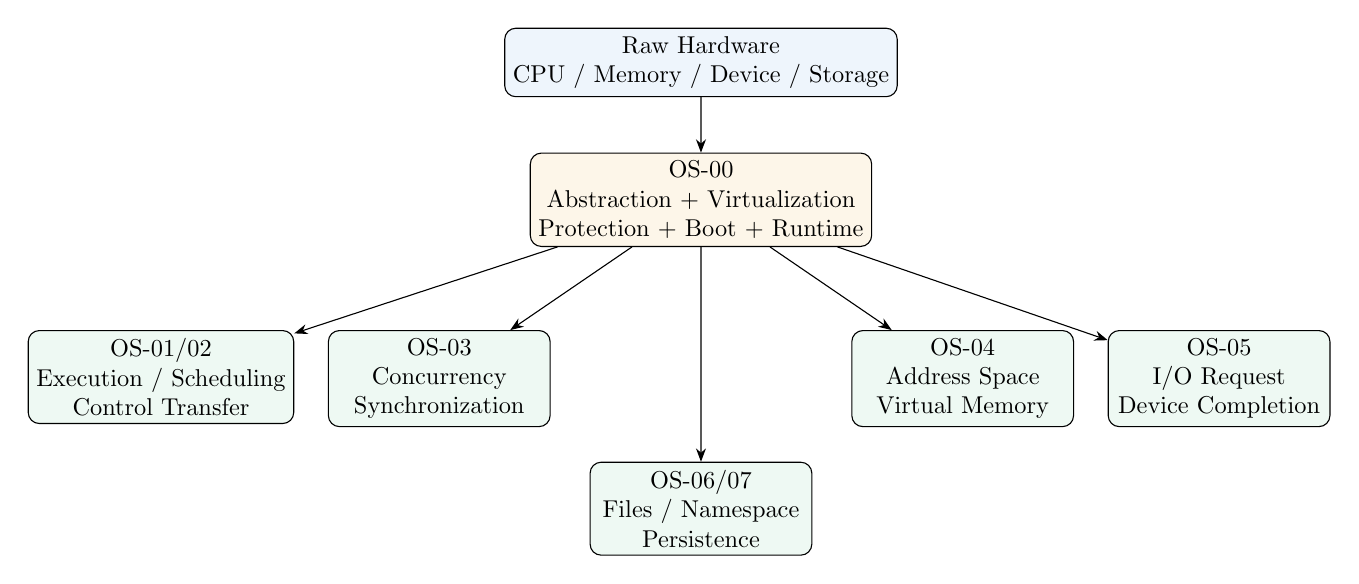
\begin{tikzpicture}[>=Stealth,node distance=8mm and 10mm,scale=.88,transform shape]
\tikzstyle{n}=[draw,rounded corners,align=center,minimum width=32mm,minimum height=9mm]
\node[n,fill=softblue] (raw) {Raw Hardware\\CPU / Memory / Device / Storage};
\node[n,below=of raw,fill=softorange] (os0) {OS-00\\Abstraction + Virtualization\\Protection + Boot + Runtime};
\node[n,below left=12mm and 34mm of os0,fill=softgreen] (p) {OS-01/02\\Execution / Scheduling\\Control Transfer};
\node[n,below left=12mm and -3mm of os0,fill=softgreen] (c) {OS-03\\Concurrency\\Synchronization};
\node[n,below right=12mm and -3mm of os0,fill=softgreen] (v) {OS-04\\Address Space\\Virtual Memory};
\node[n,below right=12mm and 34mm of os0,fill=softgreen] (io) {OS-05\\I/O Request\\Device Completion};
\node[n,below=31mm of os0,fill=softgreen] (fs) {OS-06/07\\Files / Namespace\\Persistence};
\draw[->] (raw)--(os0);
\draw[->] (os0)--(p);\draw[->](os0)--(c);\draw[->](os0)--(v);\draw[->](os0)--(io);\draw[->](os0)--(fs);
\end{tikzpicture}
\end{center}

OSTEP 三条主线也可挂回这个总图：
\[
\boxed{
\begin{aligned}
\text{Virtualization} &\Rightarrow \text{OS-01/02 + OS-04 + 部分 OS-05/06}\;\\
\text{Concurrency} &\Rightarrow \text{OS-01/02 + OS-03}\;\\
\text{Persistence} &\Rightarrow \text{OS-05 + OS-06/07}
\end{aligned}
}
\]

\section{第十章：最小调用接口——先定位层，再调用 Owner}

OS-00 只负责把问题送进正确的对象层和后续 Owner。第一观察点是：\kw{当前谈的是物理资源、受保护机制、OS 抽象、程序可见对象，还是某个已经进入细节的局部子系统？} 一旦题目开始要求进程状态、同步、页表、I/O 或文件系统内部推演，就停止在本册展开。

完整的概念辨析、七问定位与 Owner 路由统一进入同目录训练文档 \texttt{基础概念与Owner定位.md}；Canonical 继续保留 abstraction、virtualization、protection、程序运行环境与启动/结构机制本身。

\subsection{忘掉名词时怎样重新推出来？}

OS-00 最重要的不是背十几个定义，而是保留一条生成链：
\[
\boxed{
\begin{aligned}
\text{Hardware is finite / complex / shared}\;&\Rightarrow\;\text{Need abstraction and management}\\
\text{Programs must coexist}\;&\Rightarrow\;\text{Need virtualization + protection + policy}\\
\text{Activities interleave}\;&\Rightarrow\;\text{Concurrency + asynchrony problems}\\
\text{Programs start from static files}\;&\Rightarrow\;\text{Link + Load + Runtime Image}\\
\text{OS itself is software}\;&\Rightarrow\;\text{Need bootstrapping}\\
\text{Kernel is trusted}\;&\Rightarrow\;\text{Need a privilege boundary and an architecture choice}\\
\text{Whole OS may itself be virtualized}\;&\Rightarrow\;\text{Need VMM / Hypervisor}
\end{aligned}
}
\]

\begin{corebox}[本册最终心智模型]
看到“操作系统”时，不再只想到“管理软硬件资源”。应该自动看到四层：
\[
\boxed{
\begin{aligned}
\text{Physical Resource}
&\rightarrow \text{Protected OS Mechanism}\\
&\rightarrow \text{Managed Abstraction}
\rightarrow \text{Program-visible Environment}
\end{aligned}
}
\]
然后继续追问：
\[
\boxed{\text{谁共享？谁隔离？谁决策？什么时候绑定？控制权现在在哪一层？}}
\]
只要题目进入某个局部机制，就切换到对应 Topic；OS-00 的职责是\kw{把问题送到正确的 Owner，而不是把所有 OS 知识都重讲一遍}。
\end{corebox}

\section*{参考与工程边界来源}
\addcontentsline{toc}{section}{参考与工程边界来源}
\begin{itemize}
  \item Remzi H. Arpaci-Dusseau, Andrea C. Arpaci-Dusseau, \emph{Operating Systems: Three Easy Pieces}, Version 1.10：Introduction、Virtualization、Concurrency、Persistence、Virtual Machines。
  \item System V Application Binary Interface, ELF：\emph{Program Loading and Dynamic Linking}。用于 executable/shared object、process image 与 dynamic linker 的工程边界。
  \item GNU Binutils, \code{ld} documentation：链接器的 symbol resolution / relocation 基础语义。
  \item UEFI Specification 2.10, Chapter 3 \emph{Boot Manager}：firmware boot manager 与 OS loader 的启动边界。
  \item Linux Kernel Documentation, x86 boot protocol：bootloader 与 kernel entry 的工程实例。
  \item seL4 Documentation / FAQ：microkernel minimal privileged core、user-level services 与 capability-based protection 的工程边界。
  \item MIT Exokernel research：separating protection from management、application-level resource management 的经典思想。
  \item 2026 计算机学科专业基础综合（408）考试大纲：操作系统基础、程序运行环境、OS 结构、引导与虚拟机范围。
\end{itemize}

\end{document}
